\section[Resultados Adicionales]{Resultados Adicionales}

% ==================== CASO 01 ====================
\subsection{Caso 01: Problema de Hill}

\begin{frame}{Anexo \thesection\ — Caso 01: Evolución del Fitness}
    \vspace{0.1cm}
    \begin{center}
        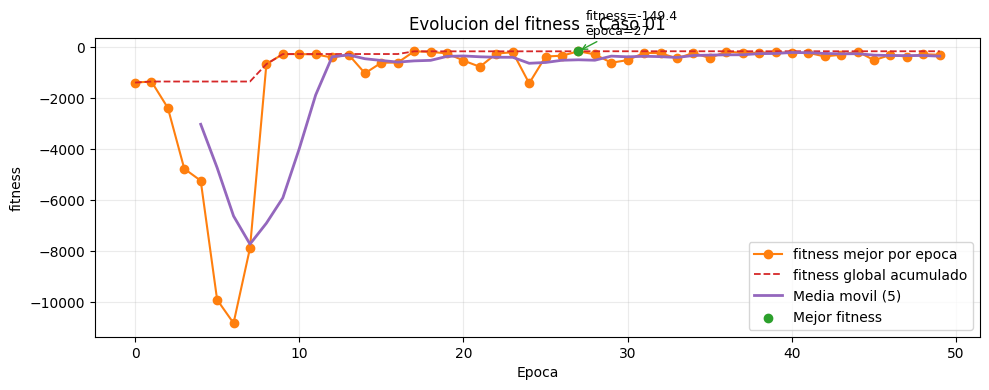
\includegraphics[width=0.85\textwidth, height=0.70\textheight, keepaspectratio]{img/resultados/caso01-evolucion_fitness.png}
    \end{center}
    \vspace{0.2cm}
    {\small Evolución del valor de fitness durante las épocas de optimización.~\textit{Autoría Propia}}
\end{frame}

\begin{frame}{Anexo \thesection\ — Caso 01: Trayectoria 3D}
    \vspace{0.1cm}
    \begin{center}
        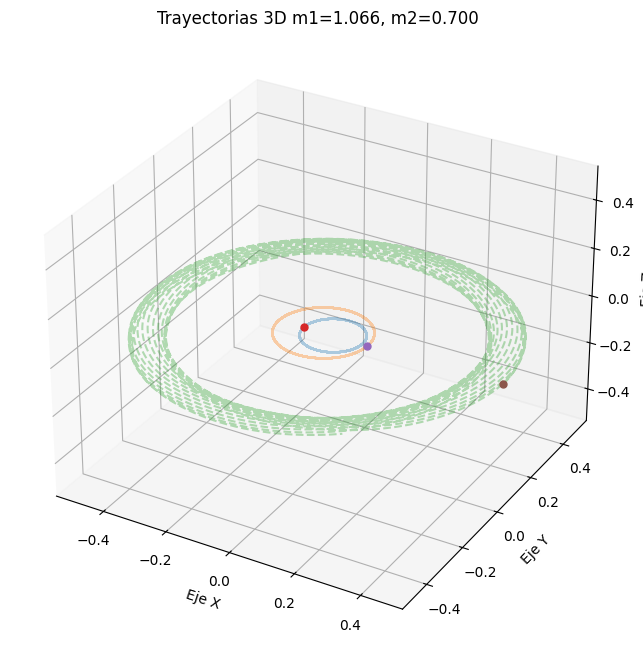
\includegraphics[width=0.85\textwidth, height=0.70\textheight, keepaspectratio]{img/resultados/caso01-trayectoria_3d.png}
    \end{center}
    \vspace{0.2cm}
    {\small Representación tridimensional de la trayectoria del sistema.~\textit{Autoría Propia}}
\end{frame}

\begin{frame}{Anexo \thesection\ — Caso 01: Vistas de Trayectoria}
    \vspace{0.1cm}
    \begin{center}
        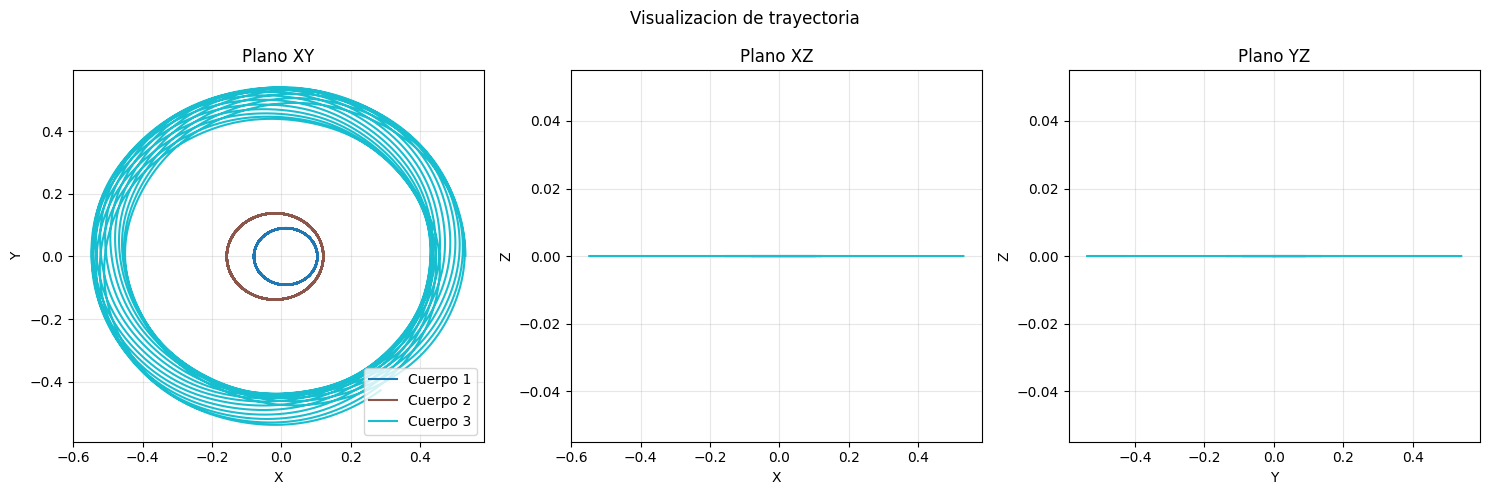
\includegraphics[width=0.85\textwidth, height=0.70\textheight, keepaspectratio]{img/resultados/caso01-vistas_trayectoria.png}
    \end{center}
    \vspace{0.2cm}
    {\small Múltiples vistas de las trayectorias del sistema optimizado.~\textit{Autoría Propia}}
\end{frame}

\begin{frame}{Anexo \thesection\ — Caso 01: Divergencia de Trayectorias}
    \vspace{0.1cm}
    \begin{center}
        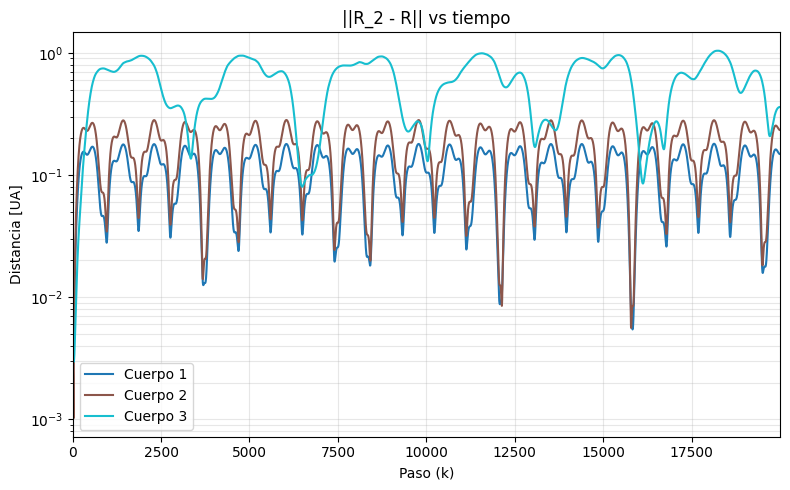
\includegraphics[width=0.85\textwidth, height=0.70\textheight, keepaspectratio]{img/resultados/caso01-comparativa_posicion.png}
    \end{center}
    \vspace{0.2cm}
    {\small Distancia entre trayectorias en función del tiempo, mostrando menor divergencia con masas optimizadas.~\textit{Autoría Propia}}
\end{frame}

% ==================== CASO 02 ====================
\subsection{Caso 02: Problema de Sitnikov}

\begin{frame}{Anexo \thesection\ — Caso 02: Evolución del Fitness}
    \vspace{0.1cm}
    \begin{center}
        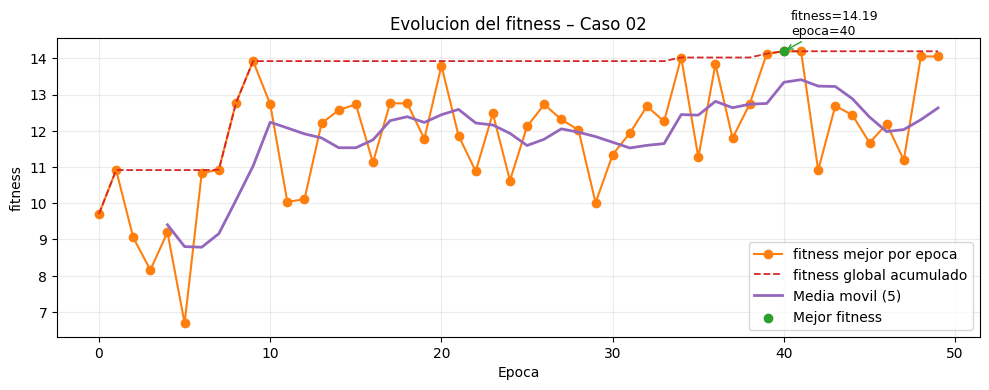
\includegraphics[width=0.85\textwidth, height=0.70\textheight, keepaspectratio]{img/resultados/caso02-evolucion_fitness.png}
    \end{center}
    \vspace{0.2cm}
    {\small Evolución del valor de fitness durante las épocas de optimización.~\textit{Autoría Propia}}
\end{frame}

\begin{frame}{Anexo \thesection\ — Caso 02: Trayectoria 3D}
    \vspace{0.1cm}
    \begin{center}
        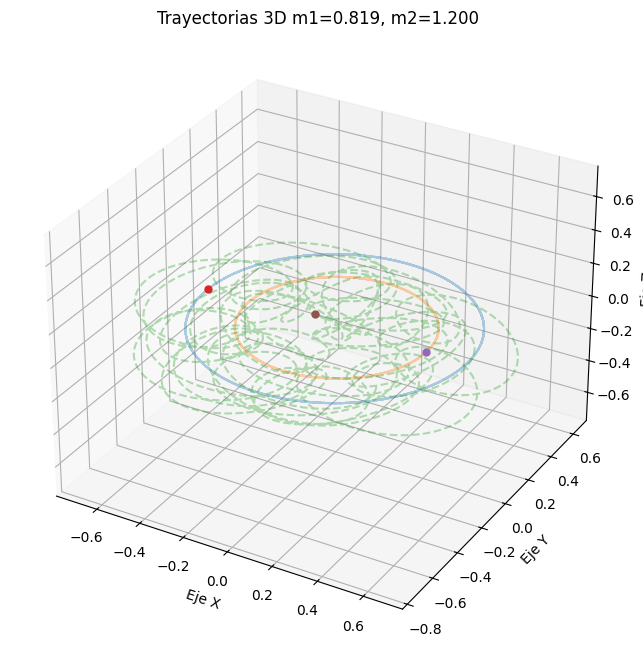
\includegraphics[width=0.85\textwidth, height=0.70\textheight, keepaspectratio]{img/resultados/caso02-trayectoria_3d.png}
    \end{center}
    \vspace{0.2cm}
    {\small Representación tridimensional de la trayectoria del sistema.~\textit{Autoría Propia}}
\end{frame}

\begin{frame}{Anexo \thesection\ — Caso 02: Vistas de Trayectoria}
    \vspace{0.1cm}
    \begin{center}
        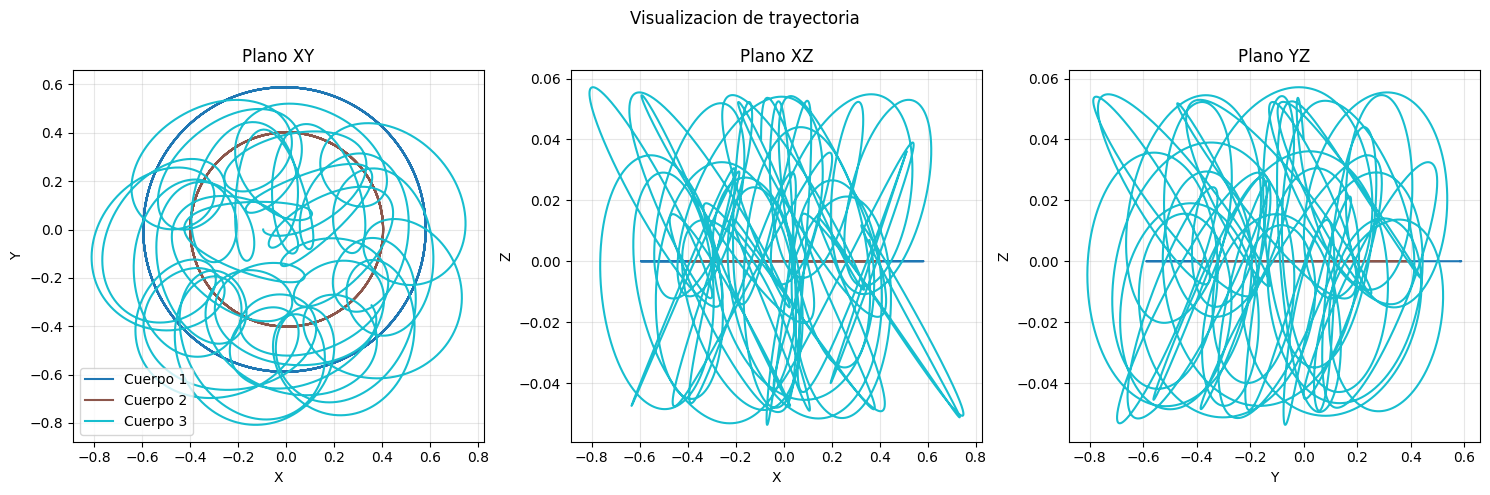
\includegraphics[width=0.85\textwidth, height=0.70\textheight, keepaspectratio]{img/resultados/caso02-vistas_trayectoria.png}
    \end{center}
    \vspace{0.2cm}
    {\small Múltiples vistas de las trayectorias del sistema optimizado.~\textit{Autoría Propia}}
\end{frame}

\begin{frame}{Anexo \thesection\ — Caso 02: Divergencia de Trayectorias}
    \vspace{0.1cm}
    \begin{center}
        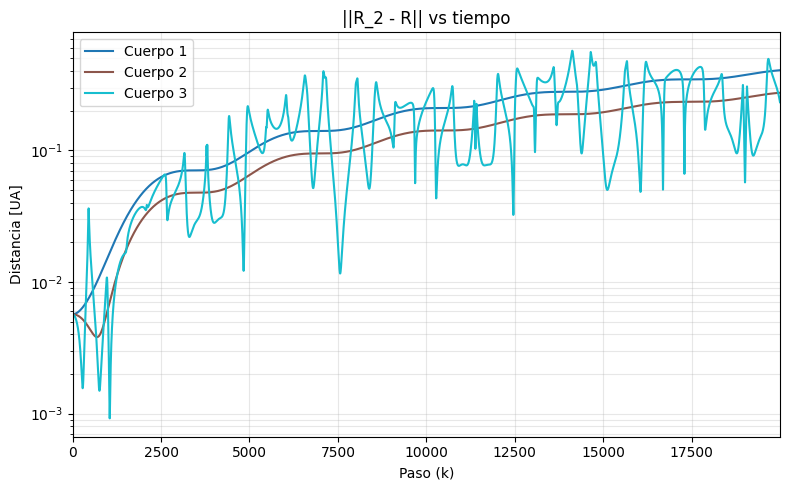
\includegraphics[width=0.85\textwidth, height=0.70\textheight, keepaspectratio]{img/resultados/caso02-comparativa_posicion.png}
    \end{center}
    \vspace{0.2cm}
    {\small Distancia entre trayectorias: el tercer cuerpo conserva cuasiperiodicidad con menos vueltas.~\textit{Autoría Propia}}
\end{frame}

% ==================== CASO 03 ====================
\subsection{Caso 03: Kepler pateado}

\begin{frame}{Anexo \thesection\ — Caso 03: Evolución del Fitness}
    \vspace{0.1cm}
    \begin{center}
        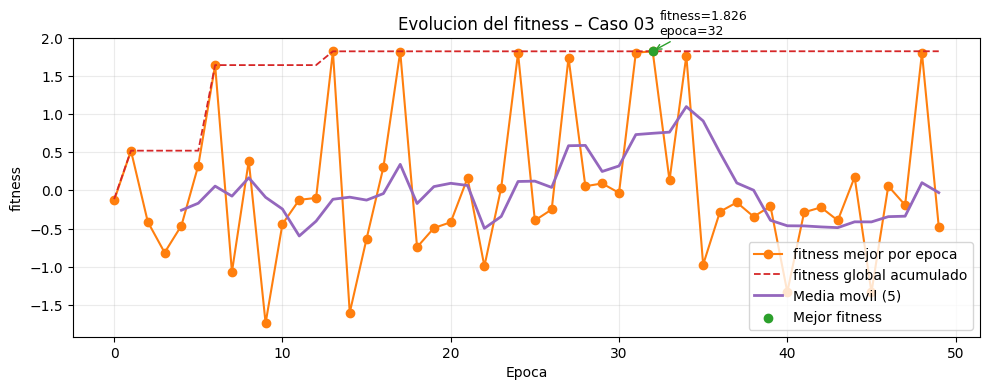
\includegraphics[width=0.85\textwidth, height=0.70\textheight, keepaspectratio]{img/resultados/caso03-evolucion_fitness.png}
    \end{center}
    \vspace{0.2cm}
    {\small Evolución del valor de fitness durante las épocas de optimización.~\textit{Autoría Propia}}
\end{frame}

\begin{frame}{Anexo \thesection\ — Caso 03: Trayectoria 3D}
    \vspace{0.1cm}
    \begin{center}
        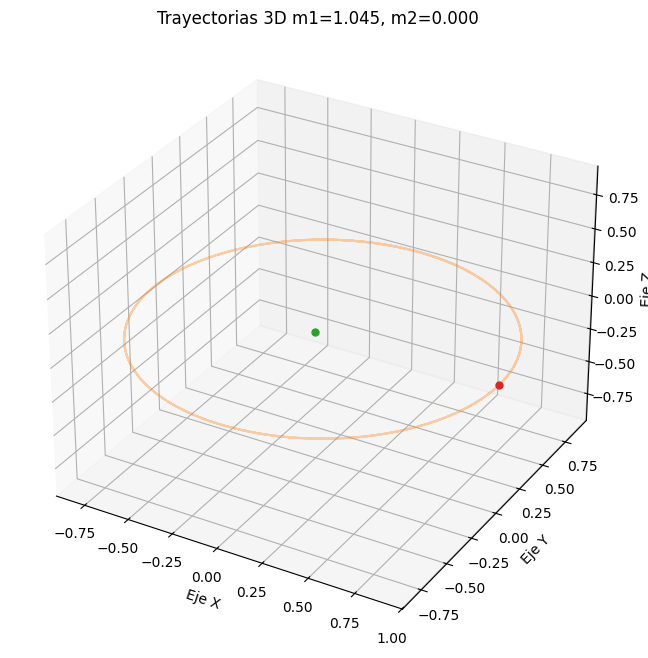
\includegraphics[width=0.85\textwidth, height=0.70\textheight, keepaspectratio]{img/resultados/caso03-trayectoria_3d.png}
    \end{center}
    \vspace{0.2cm}
    {\small Representación tridimensional de la trayectoria del sistema.~\textit{Autoría Propia}}
\end{frame}

\begin{frame}{Anexo \thesection\ — Caso 03: Vistas de Trayectoria}
    \vspace{0.1cm}
    \begin{center}
        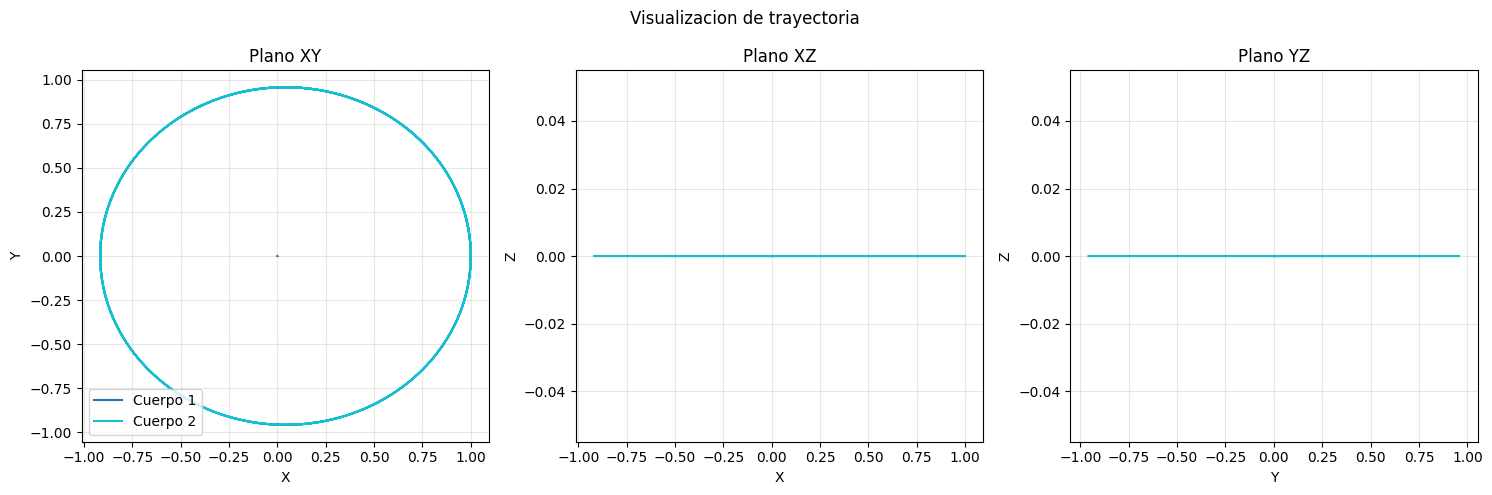
\includegraphics[width=0.85\textwidth, height=0.70\textheight, keepaspectratio]{img/resultados/caso03-vistas_trayectoria.png}
    \end{center}
    \vspace{0.2cm}
    {\small Múltiples vistas de las trayectorias del sistema optimizado.~\textit{Autoría Propia}}
\end{frame}

\begin{frame}{Anexo \thesection\ — Caso 03: Divergencia de Trayectorias}
    \vspace{0.1cm}
    \begin{center}
        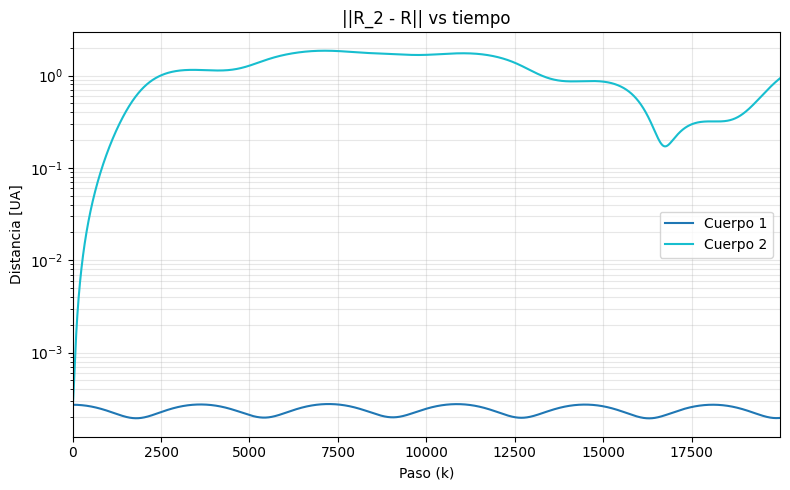
\includegraphics[width=0.85\textwidth, height=0.70\textheight, keepaspectratio]{img/resultados/caso03-comparativa_posicion.png}
    \end{center}
    \vspace{0.2cm}
    {\small Distancia entre trayectorias mostrando mejor alineación del centro dinámico con la estrella.~\textit{Autoría Propia}}
\end{frame}

% ==================== CASO 04 ====================
\subsection{Caso 04: Sistema binario con intruso}

\begin{frame}{Anexo \thesection\ — Caso 04: Evolución del Fitness}
    \vspace{0.1cm}
    \begin{center}
        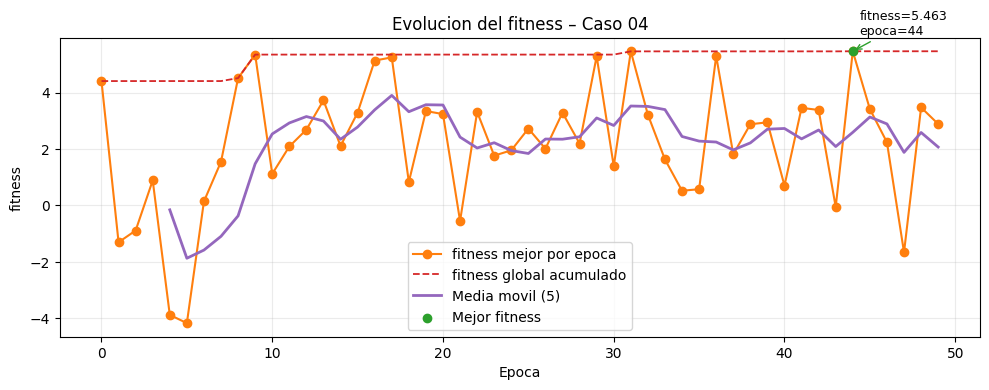
\includegraphics[width=0.85\textwidth, height=0.70\textheight, keepaspectratio]{img/resultados/caso04-evolucion_fitness.png}
    \end{center}
    \vspace{0.2cm}
    {\small Evolución del valor de fitness durante las épocas de optimización.~\textit{Autoría Propia}}
\end{frame}

\begin{frame}{Anexo \thesection\ — Caso 04: Trayectoria 3D}
    \vspace{0.1cm}
    \begin{center}
        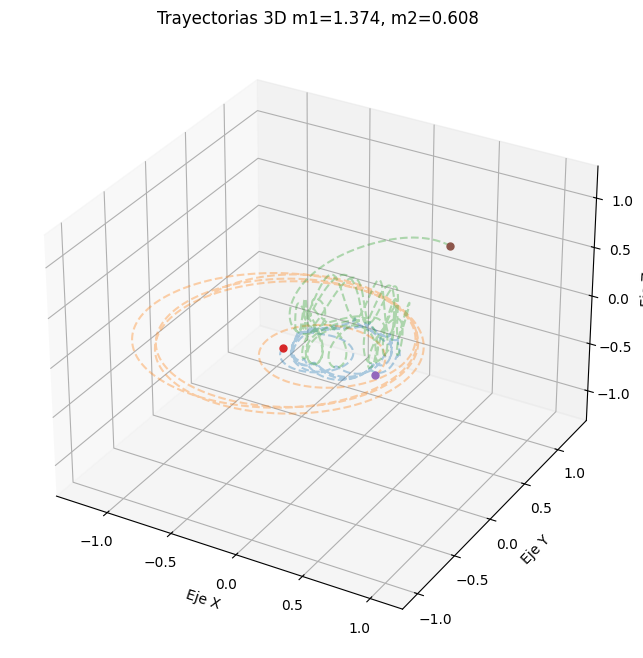
\includegraphics[width=0.85\textwidth, height=0.70\textheight, keepaspectratio]{img/resultados/caso04-trayectoria_3d.png}
    \end{center}
    \vspace{0.2cm}
    {\small Representación tridimensional de la trayectoria del sistema.~\textit{Autoría Propia}}
\end{frame}

\begin{frame}{Anexo \thesection\ — Caso 04: Vistas de Trayectoria}
    \vspace{0.1cm}
    \begin{center}
        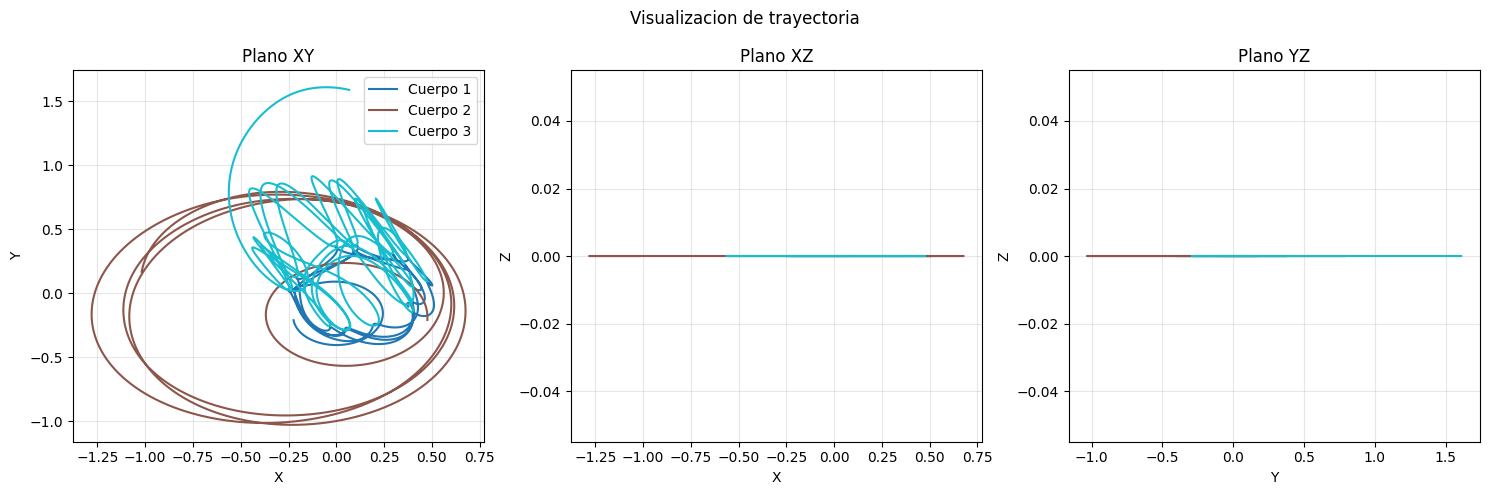
\includegraphics[width=0.85\textwidth, height=0.70\textheight, keepaspectratio]{img/resultados/caso04-vistas_trayectoria.png}
    \end{center}
    \vspace{0.2cm}
    {\small Múltiples vistas de las trayectorias del sistema optimizado.~\textit{Autoría Propia}}
\end{frame}

\begin{frame}{Anexo \thesection\ — Caso 04: Divergencia de Trayectorias}
    \vspace{0.1cm}
    \begin{center}
        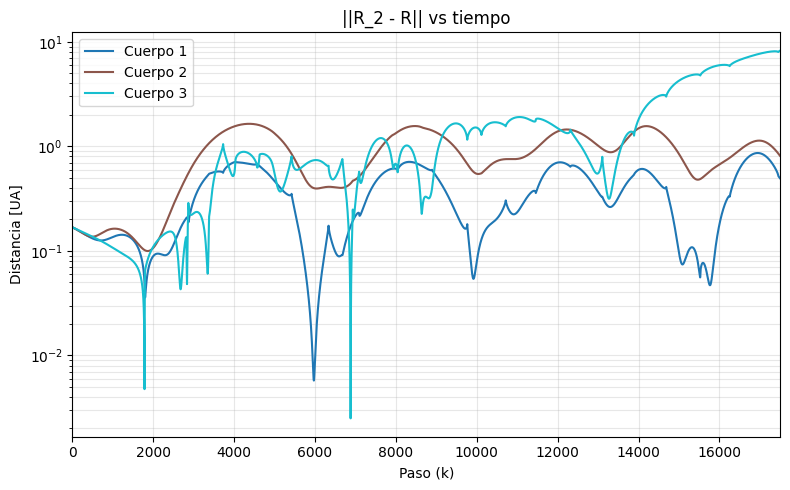
\includegraphics[width=0.85\textwidth, height=0.70\textheight, keepaspectratio]{img/resultados/caso04-comparativa_posicion.png}
    \end{center}
    \vspace{0.2cm}
    {\small Distancia entre trayectorias: con masas optimizadas el intruso permanece orbitando establemente.~\textit{Autoría Propia}}
\end{frame}

% ==================== RENDIMIENTO COMPUTACIONAL ====================
\subsection{Rendimiento Computacional}

\begin{frame}{Anexo \thesection\ — Rendimiento Computacional de los 4 Casos}
    \vspace{0.1cm}
    \begin{columns}
        \begin{column}{0.5\textwidth}
            \centering
            {\footnotesize Caso 01: Problema de Hill}\\
            \vspace{0.1cm}
            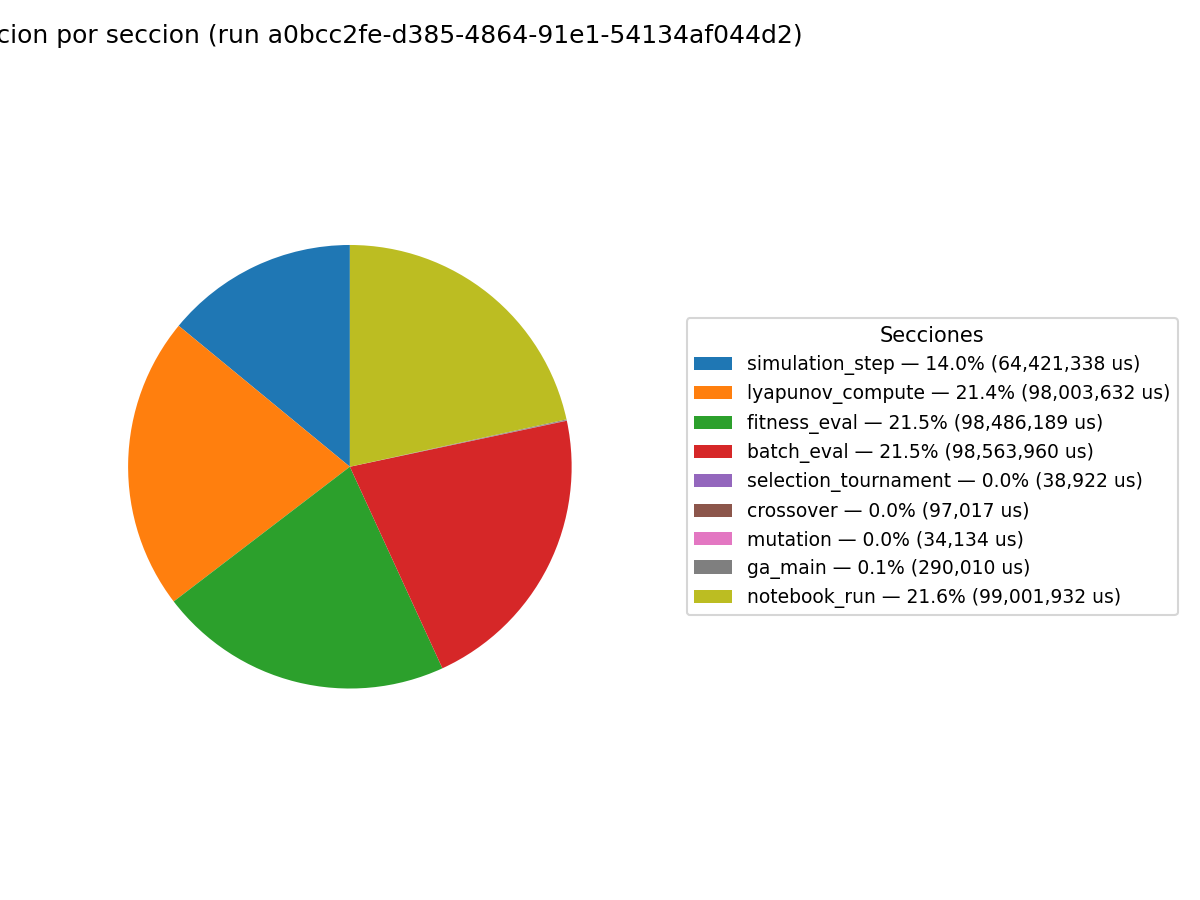
\includegraphics[width=\textwidth, height=0.3\textheight, keepaspectratio]{img/resultados/caso01-metricasTiempo.png}

            \vspace{0.25cm}
            {\footnotesize Caso 02: Problema de Sitnikov}\\
            \vspace{0.1cm}
            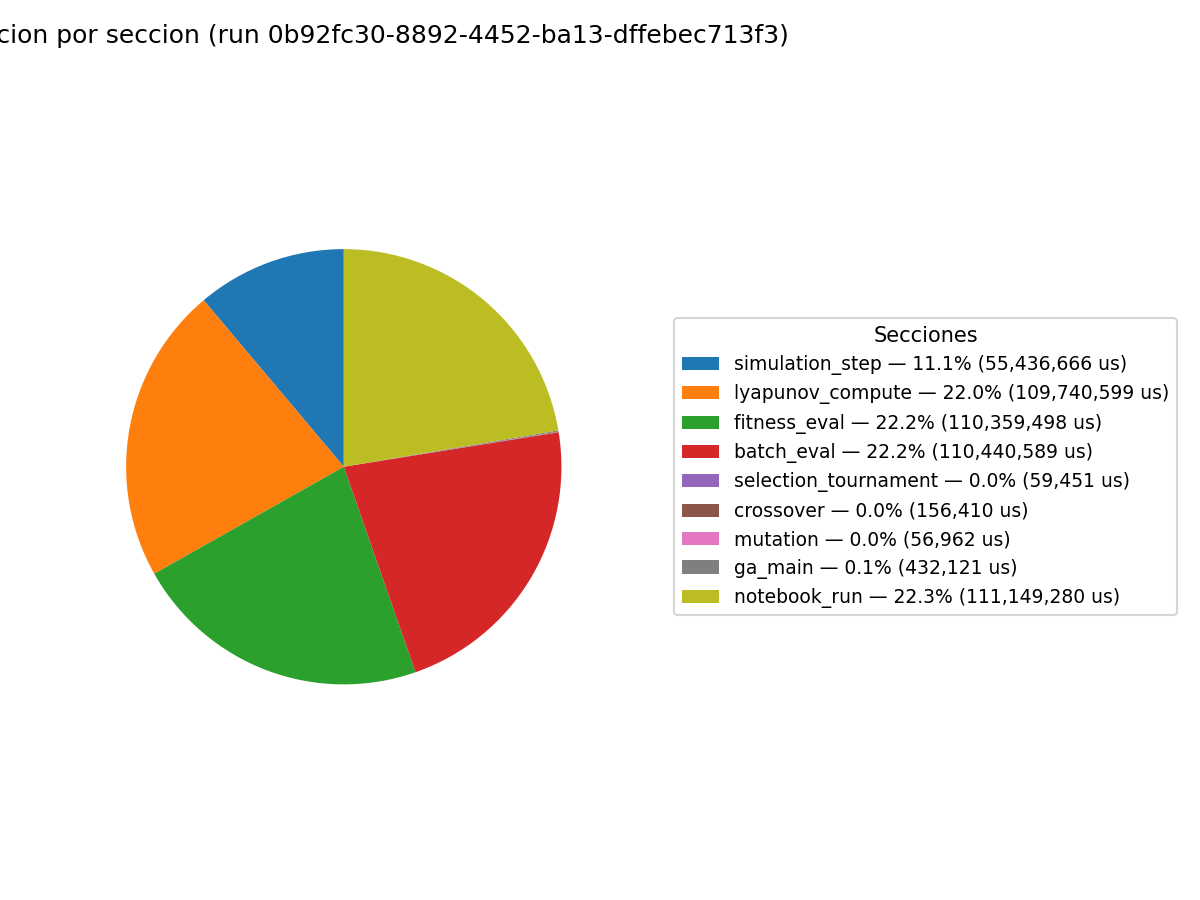
\includegraphics[width=\textwidth, height=0.3\textheight, keepaspectratio]{img/resultados/caso02-metricasTiempo.png}
        \end{column}
        \begin{column}{0.5\textwidth}
            \centering
            {\footnotesize Caso 03: Kepler pateado}\\
            \vspace{0.1cm}
            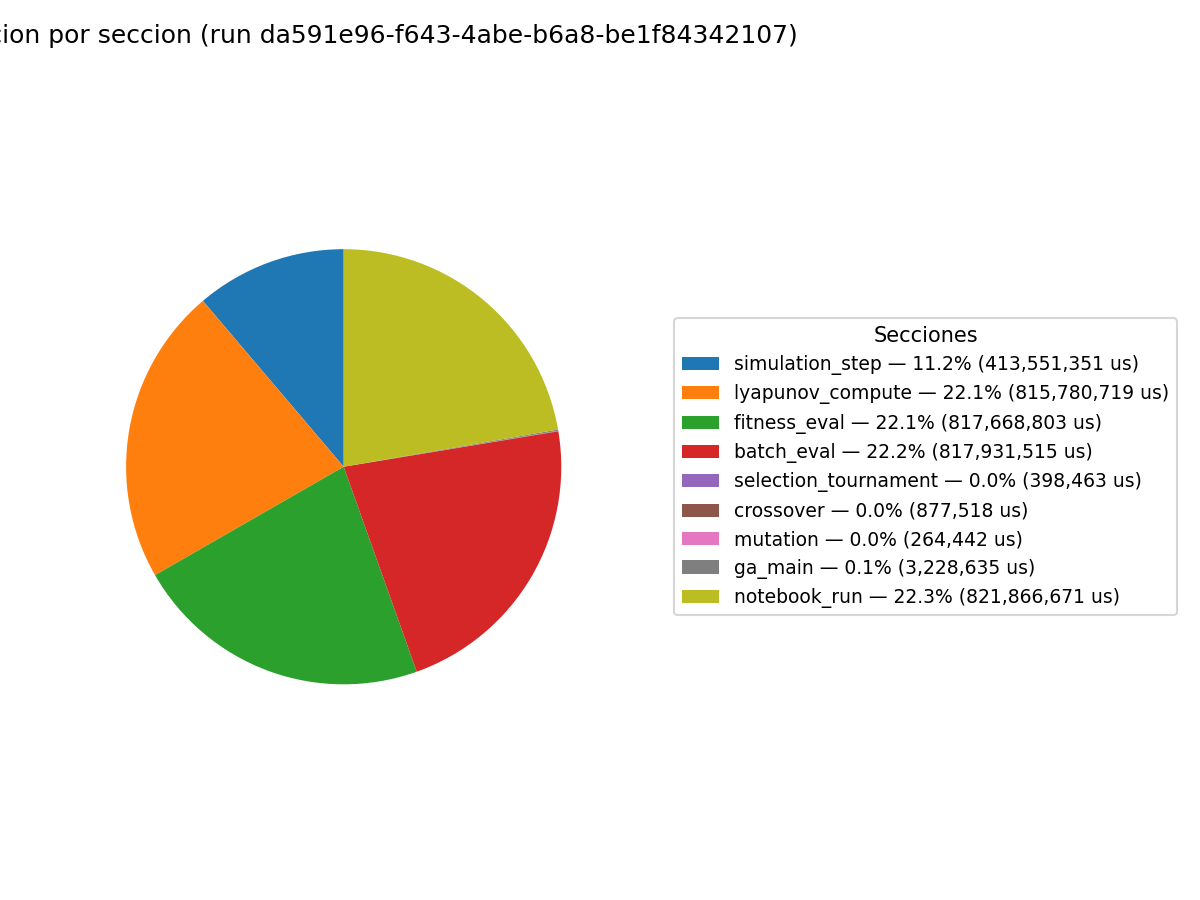
\includegraphics[width=\textwidth, height=0.3\textheight, keepaspectratio]{img/resultados/caso03-metricasTiempo.png}

            \vspace{0.25cm}
            {\footnotesize Caso 04: Sistema binario con intruso}\\
            \vspace{0.1cm}
            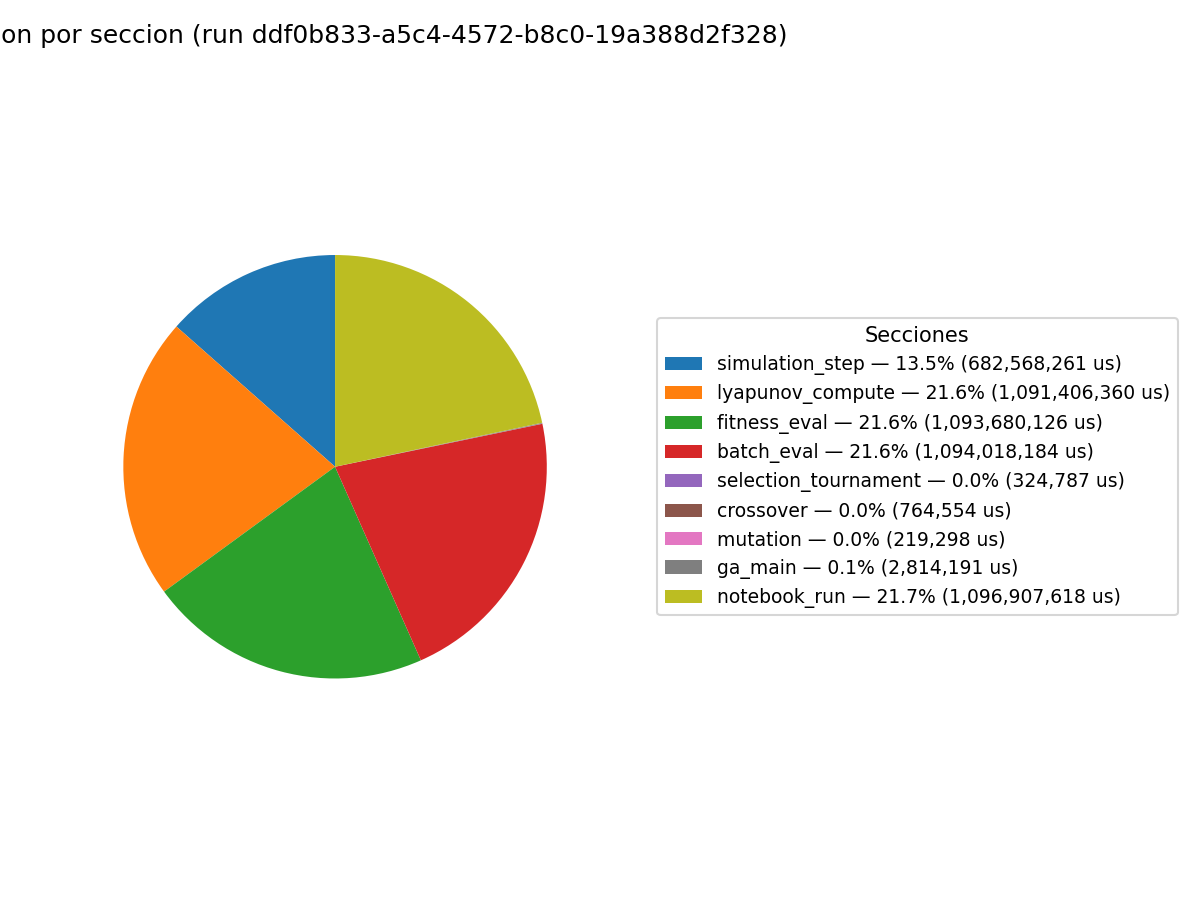
\includegraphics[width=\textwidth, height=0.3\textheight, keepaspectratio]{img/resultados/caso04-metricasTiempo.png}
        \end{column}
    \end{columns}
    \vspace{0.1cm}
    {\small Análisis comparativo de tiempos de ejecución para los 4 casos de prueba.~\textit{Autoría Propia}}
\end{frame}
